\section{块重构模型}
\label{sec:rd-block-model}

“至少需要多少描述”要先说清比较的是哪些方案。第~\ref{chap:quantization}章的量化器一次处理一个值，而开头的问题允许把许多天的记录合在一起描述。合在一起之后，一个消息对应一整块重构，失真也要按整块来算。这一节把块编码、码率与失真写成确定的对象，再用块长增长的方案序列定义什么叫“可以做到”。

\paragraph{信源与失真}
设信源依次产生$X_1,X_2,\dots$，它们相互独立，都服从取值空间$\mathcal{X}$上的同一分布$P_X$，这样的信源称为\term{无记忆信源}（memoryless source）。接收方用\term{重构字母表}（reconstruction alphabet）$\hat{\mathcal{X}}$中的值重构，它不必与$\mathcal{X}$相同。与第~\ref{chap:quantization}章一样，重构的好坏由一个失真函数$d:\mathcal{X}\times\hat{\mathcal{X}}\to[0,\infty)$衡量，$d(x,\hat{x})$是把$x$重构成$\hat{x}$的代价。

本章常用两种失真。二元或有限字母表上取$\mathcal{X}=\hat{\mathcal{X}}$，并取
\begin{equation}
  d(x,\hat{x})=\mathbf{1}_{\{x\neq\hat{x}\}},
  \label{eq:rd-hamming}
\end{equation}
它只记对错，称为\term{Hamming失真}（Hamming distortion），平均失真就是重构错误的比例。实值信源取平方失真$d(x,\hat{x})=(x-\hat{x})^{2}$，平均失真就是均方误差。

把$n$个符号合成一块$x^{n}=(x_1,\dots,x_n)$，重构块记为$\hat{x}^{n}$。块的失真取逐符号失真的平均：
\begin{equation}
  d_n(x^{n},\hat{x}^{n})=\frac{1}{n}\sum_{i=1}^{n}d(x_i,\hat{x}_i).
  \label{eq:rd-block-distortion}
\end{equation}
这种按符号相加的失真称为可分失真。取平均而不取总和，是为了让不同块长的方案在“每个符号的失真”上可以直接比较。

\paragraph{块编码}
发送方看到整块$x^{n}$后，只向接收方传一个消息编号；接收方只凭这个编号输出整块重构。图~\ref{fig:rd-block-scheme}画出了这条链路。

\begin{definition}[块编码与码率]
\label{def:rd-block-code}
一个$(n,M)$\term{率失真码}（rate-distortion code）由编码器$f_n:\mathcal{X}^{n}\to\{1,\dots,M\}$与解码器$g_n:\{1,\dots,M\}\to\hat{\mathcal{X}}^{n}$组成。$g_n$的$M$个输出称为码字，它们的集合称为码本。码的码率与期望失真分别是
\begin{equation}
  R=\frac{\log_2M}{n},\qquad
  \mathbb{E}\bigl[d_n\bigl(X^{n},g_n(f_n(X^{n}))\bigr)\bigr],
  \label{eq:rd-rate}
\end{equation}
码率的单位是bit每源符号。
\end{definition}

\begin{BookInlineFigure}
  \centering
  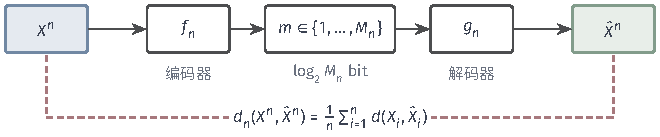
\includegraphics[width=112mm]{figures/07-probability/05-source-coding/tikz/rd-block-scheme/figure.pdf}
  \caption{块重构模型。蓝框是长度为$n$的源块，绿框是重构块。编码器$f_n$把整块映射成$M_n$个编号之一，编号要用约$\log_2M_n$\,bit描述；解码器$g_n$只凭编号输出整块重构。红色虚线表示按式~\eqref{eq:rd-block-distortion}逐符号比较两块。}
  \label{fig:rd-block-scheme}
\end{BookInlineFigure}

$M$不必是$2$的幂。把很多个块连起来发送时，$k$个编号一共有$M^{k}$种组合，用$\lceil k\log_2M\rceil$个bit就能区分，所以$\log_2M$正是每块平均要付出的bit数，除以$n$得到每个源符号的份额。码率只数编号的个数，不涉及编号怎样写成二进制串，也不对编号再作第~\ref{chap:lossless-coding}章的变长压缩；本章所说的码率都是这种固定描述的码率。

码本一旦固定，编码器怎么选最好？对每个$x^{n}$，期望失真中它的那一项是$d_n(x^{n},g_n(f_n(x^{n})))$，只依赖它被送到哪个码字。把每个$x^{n}$送到使$d_n$最小的码字，就同时使每一项最小，期望失真自然最小。所以在给定码本时，最优编码器就是\term{最近码字编码器}（nearest-codeword encoder），一个码本就决定了整个码。这与第~\ref{chap:quantization}章固定重构值后按最近邻划分区域是同一件事，只是“点”换成了整块。

\paragraph{几个简单的码}
回到开头的雨天记录：$X_i\sim\operatorname{Bern}(0.3)$，$1$表示下雨，用Hamming失真。最省的做法是不传任何信息，接收方一律猜“不下雨”。这时$M=1$，码率为$0$，错误比例是下雨的概率：
\[
  R=0,\qquad \mathbb{E}d_n=\mathbb{P}(X_i=1)=0.3 .
\]
另一个极端是逐天照传，$n=1$，$M=2$，码率为$1$，失真为$0$。

块长$n=3$时，可以只用两个码字$\{000,111\}$。在最近码字编码下，一块里$1$的个数$K$不超过$1$时送$000$，否则送$111$，这就是多数表决。$K\sim\operatorname{Bin}(3,0.3)$，
\[
  \begin{gathered}
  \mathbb{P}(K=0)=0.343,\quad \mathbb{P}(K=1)=0.441,\\
  \mathbb{P}(K=2)=0.189,\quad \mathbb{P}(K=3)=0.027 .
  \end{gathered}
\]
$K=1$或$K=2$时恰好错一位，$K=0$或$3$时不错，所以
\[
  \mathbb{E}d_3=\frac{1}{3}\,(0.441+0.189)=0.21,\qquad R=\frac{\log_2 2}{3}=\frac13 .
\]

图~\ref{fig:rd-hamming-cube}把这个码画在三维立方体上。八个顶点是全部源块，相邻顶点只差一位，所以沿棱走一步就是一个Hamming错误。蓝色顶点被送到$000$，黄色顶点被送到$111$，两块区域就是两个码字的最近邻区域。

\begin{BookInlineFigure}
  \centering
  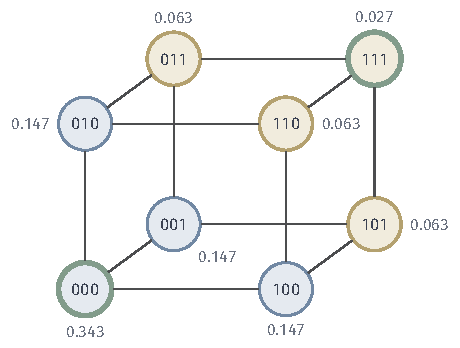
\includegraphics[width=78mm]{figures/07-probability/05-source-coding/tikz/rd-hamming-cube/figure.pdf}
  \caption{块长$3$的码本$\{000,111\}$。立方体的八个顶点是全部源块，旁边的数是它在$\operatorname{Bern}(0.3)$信源下的概率；绿色粗圈是两个码字。蓝色顶点距$000$更近，黄色顶点距$111$更近。蓝色区域的概率是$0.343+3\times0.147=0.784$，其中三个只有一位为$1$的顶点各贡献一个错误。}
  \label{fig:rd-hamming-cube}
\end{BookInlineFigure}

再换一个码本$\{000,100,010,001\}$，$M=4$，码率$\tfrac23$。$K\leq1$的块都能精确重构；$K=2$时最近码字错一位，$K=3$时错两位：
\[
  \mathbb{E}d_3=\frac{1}{3}\,(0.189\times1+0.027\times2)=0.081,\qquad R=\frac{\log_2 4}{3}=\frac23 .
\]
它把码字都放在概率大的地方，利用了“下雨少”这一规律。

还有一种不需要新码本的组合办法。把长块的前一部分符号逐个照传、其余部分一律猜$0$：照传的比例为$\lambda$时，码率为$\lambda$，失真为$0.3(1-\lambda)$。这种在不同方案之间按比例分配符号的做法称为\term{分时}（time sharing），它在码率—失真平面上连出两点之间的线段。

图~\ref{fig:rd-simple-codes}把这些码画在一起。重复码在分时线段的上方：同样码率$\tfrac13$，分时的失真只有$0.2$。四码字的码在线段下方，同样码率$\tfrac23$，分时的失真是$0.1$，它做到了$0.081$。可见简单的组合并不总是最好，块长与码本的选择都影响结果。我们要找的是所有方案都越不过的那条边界。

\begin{BookInlineFigure}
  \centering
  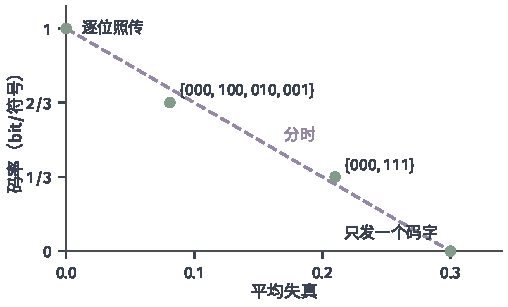
\includegraphics[width=86mm]{figures/07-probability/05-source-coding/matplotlib/rd-simple-codes/figure.pdf}
  \caption{$\operatorname{Bern}(0.3)$信源在Hamming失真下几个简单码的码率与平均失真（绿点）：只发一个码字、逐位照传、块长$3$的重复码$\{000,111\}$和码本$\{000,100,010,001\}$。紫色虚线是前两个方案之间的分时。}
  \label{fig:rd-simple-codes}
\end{BookInlineFigure}

\paragraph{渐近可达性}
单个块长的码受到整数效应的牵制：$M$只能是整数，码字只能放在格点上。为了得到一个干净的极限，我们看块长不断增长的一列码。

\begin{definition}[可达码率失真对]
\label{def:rd-achievable}
若对每个$n\geq1$都有一个$(n,M_n)$码，使
\begin{equation}
  \limsup_{n\to\infty}\frac{\log_2M_n}{n}\leq R,\qquad
  \limsup_{n\to\infty}\mathbb{E}\bigl[d_n\bigl(X^{n},g_n(f_n(X^{n}))\bigr)\bigr]\leq D,
  \label{eq:rd-achievable}
\end{equation}
则称$(R,D)$为\term{可达码率失真对}（achievable rate-distortion pair）。对给定的$D$，所有使$(R,D)$可达的$R$的下确界记为$R_{\mathrm{op}}(D)$，称为\term{操作率失真函数}（operational rate-distortion function）。
\end{definition}

定义中两个上极限分别留出了余地：码率可以比$R$稍大，只要最终不超过$R$；失真也一样。有限块长的码不在定义之内，它们只是这一列中的成员。若$(R,D)$可达，那么任何更大的$R'$与$D'$也可达，所以可达的点组成码率—失真平面中一块向右上方延伸的区域，$R_{\mathrm{op}}$是它的下边界。

\paragraph{三种失真要求}
“失真不超过$D$”还可以有别的读法，它们给出不同的极限，需要事先分清。式~\eqref{eq:rd-achievable}用的是期望失真：对源块的分布平均以后不超过$D$，个别块的失真可以很大。第二种是逐块保证，要求每一个可能的源块都满足$d_n\leq D$。第三种是超额失真概率要求，即
\[
  \mathbb{P}\bigl(d_n(X^{n},\hat{X}^{n})>D\bigr)\to0 ,
\]
允许失真超标，但超标的概率要趋于零。

若失真有上界$d_{\max}=\max_{x,\hat{x}}d(x,\hat{x})<\infty$，后两种要求都强于期望失真要求。把期望按是否超标分成两部分：
\[
  \mathbb{E}d_n\leq D\cdot\mathbb{P}(d_n\leq D)+d_{\max}\,\mathbb{P}(d_n>D)
  \leq D+d_{\max}\,\mathbb{P}(d_n>D).
\]
超额失真概率趋零时右端趋于$D$，所以满足第三种要求的码列也满足期望失真要求。反过来不成立：对一半的块照传、另一半一律猜$0$的码，期望失真可以很小，超标概率却始终是$\tfrac12$。

逐块保证则可能贵得多。仍看Hamming失真与$0<D<\tfrac12$。一个码字能“照顾”到的源块，是与它相差不超过$nD$位的那些，个数至多为$\sum_{k\leq nD}\binom{n}{k}$。对$t=D/(1-D)\leq1$，二项展开给出
\[
  1=\sum_{k=0}^{n}\binom{n}{k}D^{k}(1-D)^{n-k}
  \geq\sum_{k\leq nD}\binom{n}{k}(1-D)^{n}t^{k}
  \geq\sum_{k\leq nD}\binom{n}{k}(1-D)^{n}t^{nD},
\]
这里第二个不等号用了$k\leq nD$与$t\leq1$。而$(1-D)^{n}t^{nD}=D^{nD}(1-D)^{n-nD}=2^{-nh_2(D)}$，其中$h_2(t)=-t\log_2t-(1-t)\log_2(1-t)$是二元熵。于是
\[
  \sum_{k\leq nD}\binom{n}{k}\leq2^{nh_2(D)} .
\]

要照顾到全部$2^{n}$个源块，码字个数必须满足$M_n\cdot2^{nh_2(D)}\geq2^{n}$，即
\[
  \frac{\log_2M_n}{n}\geq1-h_2(D).
\]
这个界与下雨的概率$0.3$完全无关：概率再小的块也必须被照顾。取$D=0.1$，右端为$1-h_2(0.1)\approx0.531$\,bit。第~\ref{sec:rd-binary}节将算出期望失真标准下只需约$0.412$\,bit，差别就来自是否允许罕见的块失真偏大。

逐块保证适合要防最坏情况的场合，超额失真概率适合要控制“几乎每块”的场合。本章以期望失真为共同标准，它与平均码长一样关心长期平均表现，也是第~\ref{chap:quantization}章评价量化器的标准。
